\begin{figure}
\centering
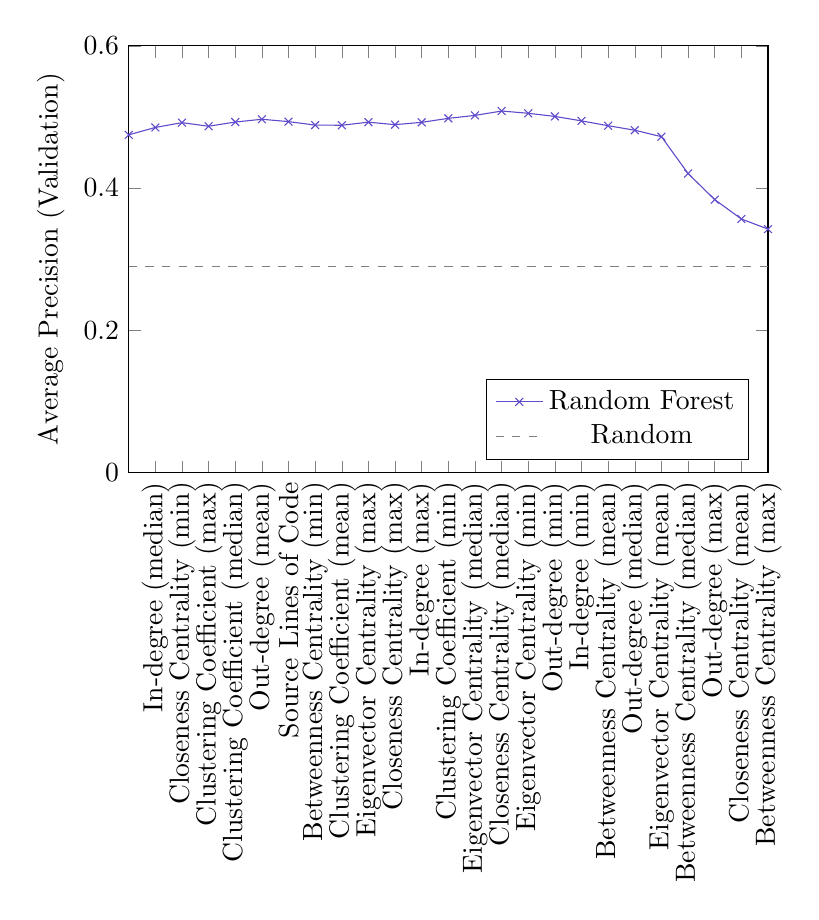
\begin{tikzpicture}
\definecolor{plotBlue}{RGB}{77,126,255}
\definecolor{plotPurple}{RGB}{97,75,202}
\definecolor{plotViolet}{RGB}{199,42,119}
\definecolor{plotOrange}{RGB}{245,80,27}
\definecolor{plotGreen}{RGB}{105,208,134}
\definecolor{plotBlack}{RGB}{0,0,0}
    \begin{axis}[
    width=0.8\textwidth,
    height=7cm,
    xlabel={},
    ylabel={Average Precision (Validation)},
    xtick=data,
    ymin=0,
    ymax=0.6,
    symbolic x coords={
\empty,
In-degree (median),
Closeness Centrality (min),
Clustering Coefficient (max),
Clustering Coefficient (median),
Out-degree (mean),
Source Lines of Code,
Betweenness Centrality (min),
Clustering Coefficient (mean),
Eigenvector Centrality (max),
Closeness Centrality (max),
In-degree (max),
Clustering Coefficient (min),
Eigenvector Centrality (median),
Closeness Centrality (median),
Eigenvector Centrality (min),
Out-degree (min),
In-degree (min),
Betweenness Centrality (mean),
Out-degree (median),
Eigenvector Centrality (mean),
Betweenness Centrality (median),
Out-degree (max),
Closeness Centrality (mean),
Betweenness Centrality (max),
    },
    xticklabel style={rotate=90},
    xmin=\empty,
    xmax=Betweenness Centrality (max),
    legend pos=south east,
    ]
    \addplot[color=plotPurple,mark=x] coordinates {
(\empty,0.4748)
(In-degree (median),0.4852)
(Closeness Centrality (min),0.4919)
(Clustering Coefficient (max),0.4869)
(Clustering Coefficient (median),0.4928)
(Out-degree (mean),0.4967)
(Source Lines of Code,0.4934)
(Betweenness Centrality (min),0.4885)
(Clustering Coefficient (mean),0.4883)
(Eigenvector Centrality (max),0.4926)
(Closeness Centrality (max),0.4891)
(In-degree (max),0.4924)
(Clustering Coefficient (min),0.4980)
(Eigenvector Centrality (median),0.5021)
(Closeness Centrality (median),0.5083)
(Eigenvector Centrality (min),0.5051)
(Out-degree (min),0.5007)
(In-degree (min),0.4944)
(Betweenness Centrality (mean),0.4876)
(Out-degree (median),0.4813)
(Eigenvector Centrality (mean),0.4722)
(Betweenness Centrality (median),0.4204)
(Out-degree (max),0.3837)
(Closeness Centrality (mean),0.3565)
(Betweenness Centrality (max),0.3422)
    };

    \addplot[mark=none,dashed,color=gray] coordinates {
        (\empty,0.29) (Betweenness Centrality (max),0.29)
    };
    \legend{Random Forest,Random};
    \end{axis}
\end{tikzpicture}
\caption{
    Average precision for best random forest model after tuning,
    when cumulatively removing features.
    In-degree (mean) remains as last feature.
}\label{fig:lint_freq_rf_feats}
\end{figure}